\documentclass{article}

% \usepackage[margin=1 in]{geometry}
\usepackage{float,mathtools,amssymb,amsthm,ifthen,url}

\newtheorem{theorem}{Theorem}
\newtheorem{lemma}{Lemma}
\newtheorem{definition}{Definition}

\newcommand{\probnum}{}
\newcommand{\probchildren}{}
\newenvironment{prob}[2][NOCHILDREN]{%
    \edef\probnum{\probnum #2}%
    \renewcommand{\probchildren}{#1}%
    \ifthenelse{\equal{#1}{NOCHILDREN}}{%
        \vspace{1em}
        \noindent%
        \begin{minipage}{\linewidth}
            \begin{center}
                \textbf{\textit{\probnum}}%
            \end{center}%
            \setlength\parindent{15pt}%
        }
        {}%
}{%
    \ifthenelse{\equal{\probchildren}{NOCHILDREN}}
        {\end{minipage}}
        {}%
}

\newcommand{\set}[2][]{
    \left\lbrace
    #2
    \ifthenelse{\equal{#1}{}}
        {}
        {\; \middle| \; #1}
    \right\rbrace
}

\title{Distributed Stockfish}
\author{Joel Kottas and Hassler Thurston}
\date{}

\begin{document}

\maketitle

\begin{abstract}
	Since 1997, when Deep Blue first beat Garry Kasparov in a chess match,
	there has been a lot of
	interest in improving existing chess engines. However, there are not
	many distributed implementations of chess engines, partly
	because there are many challenges to creating independent work to be
	done among multiple nodes. We take the world's
	best known open-source chess engine, Stockfish, and create distributed
	implementations of it which can run on a high-performance cluster. We
	discuss the challenges of implementing such a distributed system, our
	approaches to counteract these challenges, and present our sub-optimal findings.
\end{abstract}

\section{Introduction}
As of April 15, 2017, Stockfish\cite{Stockfish} is currently the top performing
chess engine in existence, and the only chess engine in the top three whose
source code is freely available\cite{ChessStandings}. The current best
performing version of Stockfish is massively parallelized but not distributed,
and we seek to explore whether a distributed implementation of Stockfish can
outperform the current state-of-the-art implementation. Under the hood,
Stockfish recursively searches chess positions using a variant of an alpha-beta
pruning algorithm, using a shared lookup table (transposition table) to
store a map between previously searched board positions and their heuristic
evaluations.

Many challenges arise when attempting to modify the
existing Stockfish algorithm to perform well on a cluster of machines.
For example, deciding how to split up the work among nodes when performing an alpha-beta game
tree search is non-trivial, as the latency of the round-trip time between nodes
may become significant. Furthermore, often a given chess position will show up
multiple times within a game tree search, and we would ideally like to not
duplicate work among nodes searching the same chess position.

We present and compare a number of distributed modifications of Stockfish
using OpenMPI\cite{OpenMPI}, an interface which allows processes in a distributed system to
send and receive messages from one another, and allows remote memory accesses
between computers. The overhead of initializing a MapReduce job and the
inherent difficulty in assigning non-overlapping board states to MapReduce tasks
makes a MapReduce implementation for this problem infeasible. In addition,
message-passing gives us greater flexibility when designing, implementing, and
comparing different distributed prototypes. These prototypes will be discussed in
the Algorithms section, and comparisons discussed in the Results section.

Unfortunately, only one of our algorithms performs as well as the original
Stockfish implementation -- the rest perform much more poorly.
The inherent difficulty
of splitting work among nodes has proven harder than originally thought, for
reasons discussed in the Algorithms and Results sections.

\section{Overview and Related Research}\label{Overview}
Given a board position in chess, an algorithm would like to return the move in
that position which maximizes winning chances. Since the total number of chess
positions is infeasible to compute~\cite{chesscom}, Stockfish uses a number of
heuristic functions to evaluate board positions, to decide which nodes to
search next, and to decide when to stop searching.
Because improving the heuristic functions is beyond the scope of this project, we do
not consider them or modify them in our implementations.
However, with the current heuristics in place and with the help of the Late Move
Reduction technique~\cite{wiki:LMR},
Stockfish is able to decrease the average branching
factor\footnote{average number of moves to search, given a board position} from
about 35 to less than two~\cite{stockfish:code}.

\begin{figure}[t]
	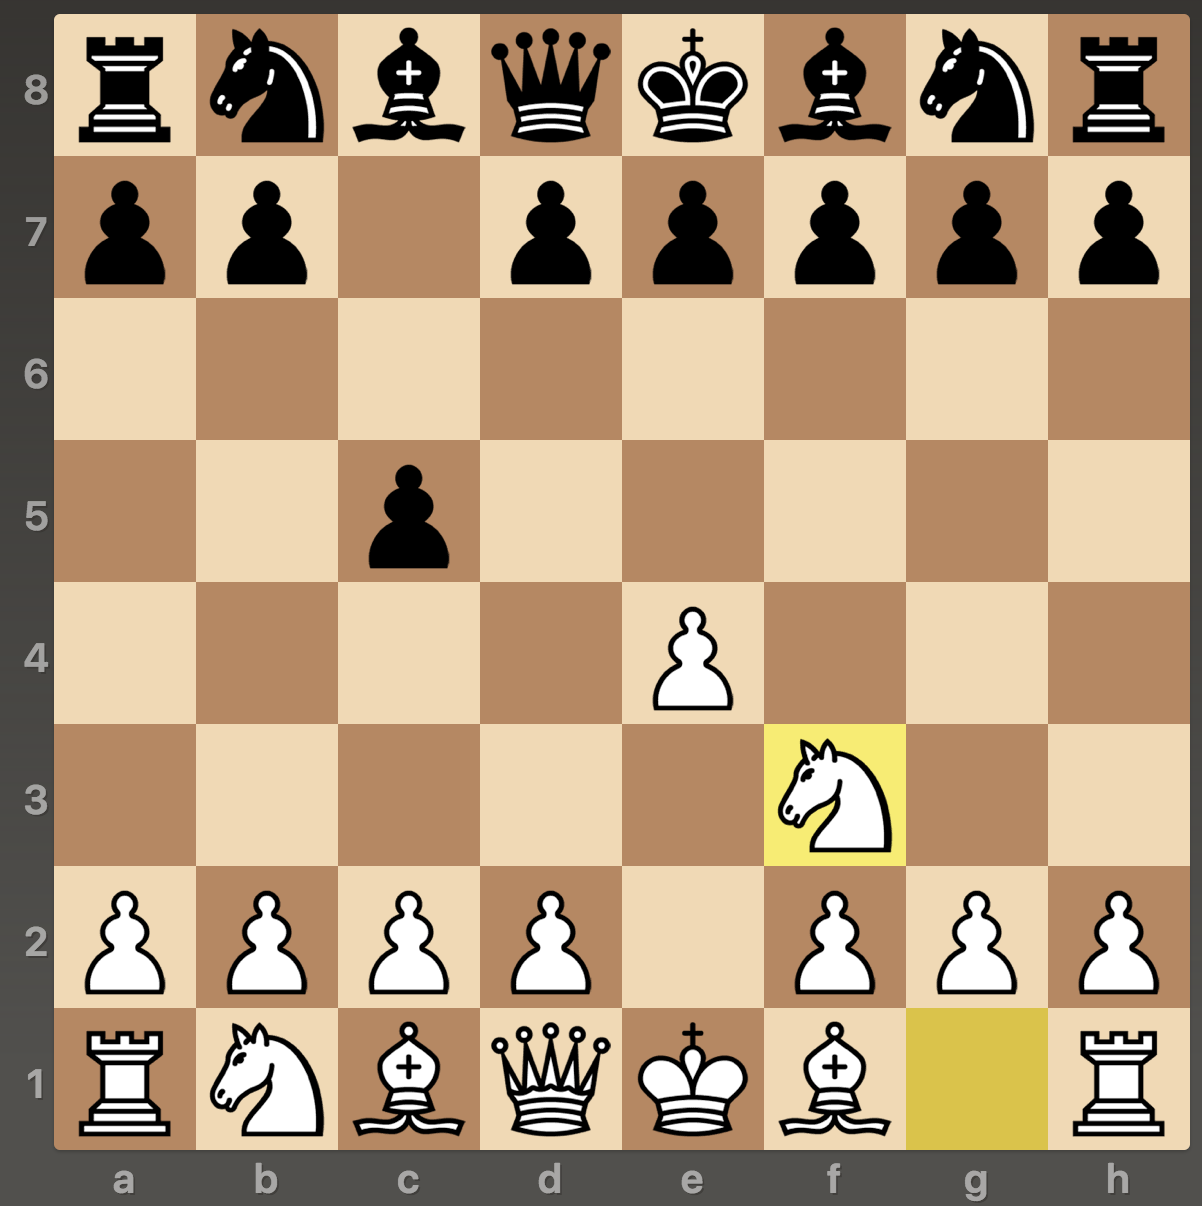
\includegraphics[width=0.5\textwidth]{transposition}
	\caption{A sample chess position which can be reached in two different
	ways: 1. e4 c5 2. Nf3, or 1. Nf3 c5 2. e4. (Figure made on
	Chess.com~\cite{chesscom:fig})}
	\label{fig:transpositions}
\end{figure}

In chess, transpositions\footnote{identical board positions which can
be reached by more than one move order} are quite common.
As can be seen in Figure~\ref{fig:transpositions}, the same game board may be
repeated in the game tree search after only three moves.
To avoid evaluating the same position
twice, Stockfish employs a transposition table, or a map from board positions to
Stockfish's evaluation of that position. The key for each board position is a lossy 64-bit
Zobrist hash\cite{Zobrist}, which has the property that the hash keys of board
positions are 
indistinguishable from a uniform distribution. Stockfish resizes its hash table
in sizes which are powers of two, and implements small separately-chained arrays
(called clusters), with each cluster size corresponding to the size of a hardware
cache line.
It is interesting to note that Stockfish chooses not to synchronize the
transposition table, instead incurring
the small probability of bogus data in its transposition table in favor of
searching positions to a greater depth in the same amount of time.

\subsection{Distributed Alpha-Beta Search}
Two primary methods have been proposed to do distributed alpha-beta search. The
Young Brothers Wait Concept (YBWC), proposed by Feldmann et.
al.~\cite{YBWC:article}, involves searching the most
promising move first (the principal variation) to establish bounds on alpha and
beta. After establishing these bounds, worker nodes may then start to examine sibling
nodes of the principal variation line, in order of decreasing depth.
Please see Figure~\ref{fig:YBWC} for more information. Young Brothers has been used
extensively since it was proposed in 1990, and was the primary parallel game tree search algorithm used in
Stockfish until January 2016. We decided not to implement a Young Brothers
distributed implementation, for the primary reason that Stockfish now uses Lazy
SMP.

\begin{figure}[t]
	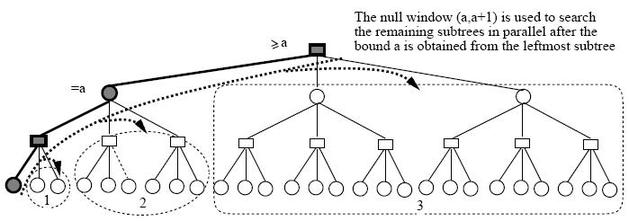
\includegraphics[width=\textwidth]{PVSplit}
	\caption{Young Brother's Wait Concept: Explore the principal variation
	first to establish bounds on alpha and beta, then explore the sibling
	nodes in parallel. Image from Gao et. al.~\cite{PVSplit:article}.}
	\label{fig:YBWC}
\end{figure}

Lazy SMP\footnote{Shared-Memory Parallelism} involves worker nodes searching the
same starting position at different depths and with different move
orders~\cite{LazySMP}.
With high probability, each worker will evaluate a given position at
slightly different times, which means that it is highly likely that
threads which access the position at slightly later times
can look up the value of that position in the transposition table. All
of our distributed implementations of Stockfish employ a variant of Lazy SMP.

\subsection{Difficulties for Distributed Chess Engines}
From our research, it seems as if distributed chess engines are much rarer than
non-distributed engines. 
As mentioned above, there tends to be a lot of duplicate work performed during
game tree search, unless workers share information about the evaluation of
particular board states. As we have seen above, Stockfish's
solution is to share an unsynchronized transposition table among threads. On
multiple nodes, we must now worry about distributing the transposition table
intelligently so as not to replicate work, and communicating results about chess positions between
nodes efficiently given the speed of the network. Alternatively, we may elect
to keep transposition tables local among nodes, but then we run the risk that
each node will be duplicating the work of other nodes.

\subsubsection{Upper Bound on Speedup}
Suppose each node can process up to $p$ unique positions per second. With $n$ nodes, we
obtain a very liberal upper bound of $p\times n$ unique positions which can be processed per
second. This is assuming that no two nodes will process the same position. In
the absence of a well-designed transposition table, this upper bound becomes
much smaller than $p \times n$. In fact, with the overhead of communication
among nodes, the true number of positions processed per second may end up being
much less than $p$. We believe the overhead involved in distributing a
transposition table has led many developers to believe that the gain in
implementing a distributed chess engine is far lower than the gain in
optimizing another facet of the engine. For example, creating a slightly
more accurate heuristic may reduce the average branching factor in alpha-beta
search by a small amount, which means the engine may need to search far fewer
positions.

\subsubsection{Transposition Table Accesses}
As part of our preliminary analysis and design, we analyzed the quantity of
read and write accesses that Stockfish threads make to the transposition table, as well as
the proportion of accesses that are reads. Figure~\ref{fig:accesses} summarizes
our results of running each benchmark test on node2x18a, for varying numbers of
thread counts. We let Stockfish run for varying amounts of time between 1
minute and 30 minutes, taking the median values for each thread count. As can be
seen, each thread writes to more than 50\% of all transposition table entries during
this time, while only reading upwards of 25\% of entries. Furthermore, the vast
majority of accesses to the shared transposition table are writes. This poses a
challenge if we would like to synchronize the transposition table, and gave us
more experimental reason to support Stockfish's original design choice of not
synchronizing the transposition table.

\begin{figure}
	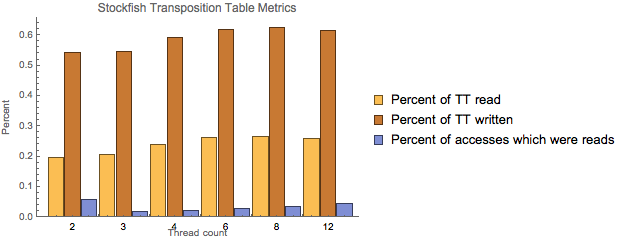
\includegraphics[width=\textwidth]{../plots/TTmetrics}
	\caption{Accesses to a 16GB shared Transposition Table, original Stockfish
	implementation. Each thread writes to a majority of slots in the
	transposition table, and the vast majority of total accesses to this
	table are writes.}
	\label{fig:accesses}
\end{figure}

Since we expect there to be many more accesses to the transposition tables in a
distributed implementation, including via MPI calls, we chose to leave the
transposition tables unsynchronized.

\subsubsection{Jonny}
Nonetheless, Jonny~\cite{wiki:Jonny} was a successful distributed chess engine
which won the 21st World Computer Chess Championships in 2015~\cite{WCCC15}.
Jonny distributed the search tasks among more than 2400 cores, and was able to
obtain a relatively small advantage over competitors in the 2015
championship~\cite{WCCC15}.
While this tells us that such a distributed implementation is possible,
unfortunately Jonny is not open-source, and we have found no details about its
implementation. As such, we are not aware of the techniques used in Jonny.

\section{Methodology}\label{Algorithms}
Using the Stockfish implementation as a base~\cite{stockfish:code},
we implemented and tested a number
of different distributed algorithms for chess game tree search. To test each
algorithm, we measured the number of milliseconds for the algorithm to finish
searching the game tree at a given depth, starting from the root position.
Stockfish does have a built-in testing framework Fishtest~\cite{fishtest:code},
which plays different versions of Stockfish against each other and evaluates
different versions on a win-draw-loss ratio. While we were able to install Fishtest 
on the csug.rochester.edu network, we were unable to run fishtest with our MPI
implementations. As such, we opted instead for the 
slightly less accurate time-to-depth heuristic.

We tested each of our models on the Infiniband cluster of machines
node03, node04, node05, and node06, on the csug.rochester.edu network.
Each of the machines has eight Intel Core i7 processors, running at 3.4GHz, with
an 8KB L1 cache. We ran each of our implementations for 60
seconds on the root position, recording the time it took for each iterative
deepening loop to complete. For each algorithm, we took the median of four 
measurements, as we would like to capture the best measure of central tendency.

The following is a description of each of our algorithms.

\subsection{Naive Transposition Table}
The Naive TT (Naive Transposition Table) algorithm works by dividing up the
transposition table into sections, with each section owned by one node. When a
given process wants to look up the value for a position, it sends an
{MPI\_RMA}\footnote{Remote Memory Access, where the receiver does not need to be active}
request to the node which may contain the transposition table entry. Once
received, the process can then determine if it needs to search the given
position, or if it can use the previous value attained by another node.

\subsection{Irreversible Transposition Table}
Given our preliminary findings in Figure~\ref{fig:accesses}, we wanted to
create a way to more effectively map board positions to nodes. As the current
Zobrist hash function maps positions to keys uniformly, there is a uniform
probability that any given transposition table lookup will go to a random node.
To improve this, note that there are some moves in chess (e.g.\ captures and pawn
moves) which are irreversible: if a pawn move takes us from A to B, position A
is always unreachable. Thus, the sets of reversible chess positions form
equivalence classes, and are likely to be near each other in an alpha-beta
search. The irreversible transposition table algorithm modifies the hash
function so that each set of reversible positions are guaranteed to map to the
same node.

\subsection{Transposition Table with Local Cache}
Note that the above two algorithms make near-constant use of the shared
interconnect between the nodes. To decrease the use of the interconnect, we
employ an additional local cache for each node, for positions which have been
computed by other nodes. We implemented a cache which can store up to 3072
transposition table entries, with three-way associativity. Each time a node
accesses a position from another node, it puts it in this cache, evicting older
or less important board positions as appropriate.

\subsection{Transposition Table with Locked Cache}
TODO

\subsection{Global Lazy SMP}
Given the success of Lazy SMP in the original Stockfish implementation, we
wanted to test the efficiency of having all worker nodes perform the Lazy SMP
algorithm, without the added overhead of requesting positions from other nodes.
In this model, each process keeps its own local transposition table, to be
shared with all threads on that process.

To communicate results between nodes,
we isolate a separate Master thread on each process to be in charge of
communication. The Master threads attempt to synchronize the transposition table
by performing a linear scan over the elements in the table, doing an
{MPI\_Allreduce} to synchronize the transposition table entries for a given
cluster of entries. Figure \ref{fig:diagram} visualizes this idea.

If a given cluster of three entries is full, {MPI\_Allreduce}
keeps the three ``most accurate'' entries, and evicts the rest. The accuracy of
a given entry is judged as a combination of its age\footnote{how long it has
been in the transposition table} and its depth\footnote{how deep from this
position is the heuristic evaluation based on}. With Global Lazy SMP, we
attempt to avoid the overhead of threads waiting on the results of a lookup from
entries on other nodes.

\section{Results} \label{Results}
asdf

\section{Conclusion}


\pagebreak
\pagestyle{empty}

\bibliographystyle{plain}
\bibliography{report}

\end{document}
